\section{Level 1.3b: Purpose-Designed Validation and Causal Intervention}
\label{sec:level13b}

\subsection{Experimental design and eight preregistered hypotheses}
\label{sec:level13b-design}

Level 1.3b's own preregistration manifest freezes eight hypotheses (H1--H8
below), the eight-label decision-gate vocabulary
(\cref{sec:decision-gate-extended}), and a purpose-designed, not
pooled-post-hoc, stage sequence, before any Stage 3+ run executed. Eleven
stages (Stage 0--10) followed, summarized here with their run counts:
Stage 0, frozen-compatibility and cross-process determinism checks (35
comparison runs); Stage 1, a hand-computed microcase plus two
representative runs; Stage 2, a 96-run ($24\times4$) bargaining-activation
calibration sweep; Stage 3, a 216-run purpose-designed matched factorial
(3 orderings $\times$ 3 entrenchment levels $\times$ 4 legitimacy
conditions $\times$ 3 ecological strata $\times$ 2 seeds); Stage 4, a
240-run homogeneous discovery pool; Stage 5, 80 runs (16+16+48) of
persistence classification and counterfactual-persistence diagnostics;
Stage 6, 72 runs (12 seeds $\times$ 6 arms) of sham-controlled causal
intervention; Stage 7, a model-comparison fit reusing Stage 4's own pool
(0 new simulation runs); Stage 8, a 96-run disjoint fresh confirmation;
Stage 9, a 240-run deterministic measurement-weighting audit (re-running
Stage 4's own seeds); and Stage 10, a 24-run ecological-control scale
check. \Cref{tab:l13b-design} summarizes the design; \Cref{tab:l13b-hypotheses}
reports every hypothesis's disposition alongside its own headline evidence.

\begin{table}[htbp]
\centering
\caption{Level 1.3b experimental design by stage.}
\label{tab:l13b-design}
\adjustbox{max width=\textwidth}{\begin{tabular}{@{}lll@{}}
\toprule
\textbf{Stage} & \textbf{Purpose} & \textbf{Runs} \\
\midrule
0 & Frozen-compatibility \& cross-process determinism & 35 (20+15 comparison) \\
1 & Hand-computed microcase \& representative runs & 2+1 \\
2 & Bargaining-activation calibration sweep & 96 (24 cells $\times$ 4 seeds) \\
3 & Purpose-designed ordering/entrenchment/legitimacy factorial & 216 \\
4 & Homogeneous discovery pool & 240 \\
5 & Persistence classification + counterfactual persistence & 80 (16+16+48) \\
6 & Sham-controlled causal history-erasure intervention & 72 (12 seeds $\times$ 6 arms) \\
7 & Discrete/continuous/path-dependent model comparison & 0 (refits Stage 4 pool) \\
8 & Disjoint fresh confirmation & 96 \\
9 & Measurement-weighting audit & 240 (deterministic re-run of Stage 4 seeds) \\
10 & Ecological-control scale check & 24 \\
\bottomrule
\end{tabular}
}
\end{table}

\subsection{H1--H2: activation and ordering}
\label{sec:level13b-h1h2}

\textbf{H1 (bargaining activation): supported.} Stage 4's own 240-run
discovery pool found 166/240 (69.2\%) of runs showing a sustained
\texttt{bargaining\_participation} activation under \texttt{repeated\_%
shocks} pressure, with all three ecological strata represented ---
neither near 0\% (the fix not working) nor near 100\% (the manipulation
uninformative). Stage 2's own calibration sweep found 20/24 (83\%) of
cells landing in the target activation range $[0.2, 0.8]$ at the
\textit{unmodified} Level 1.1/1.2b \texttt{contribution\_amount}/%
\texttt{contribution\_period\_steps} defaults --- no generative
recalibration was required. The fix itself was an observer-construction
correction (\cref{sec:level13b-limitations}), not a change to any
generative rule, confirmed by regression test
(\cref{fig:l13b-bargaining-activation}).

\textbf{H2 (ordering effect): weakly supported, with a disclosed
sign-consistency caveat.} Stage 3's 216-run matched factorial pools to
mean $S_{\text{obs}}$ of 0.597 (\texttt{security\_first}), 0.590
(\texttt{bargaining\_first}), 0.591 (\texttt{coevolution}) --- a real but
modest ($\approx1.2\%$ relative) spread; mean $Z_{\text{obs}}$ 0.369,
0.364, 0.366 ($\approx1.4\%$ relative spread). Of 108 matched pairwise
contrasts, 26 (24.1\%) show a seed-clustered bootstrap confidence interval
on the raw $S_{\text{obs}}$ difference that excludes zero, and 35 (32.4\%)
do so for $Z_{\text{obs}}$ --- a real minority effect, not a null.
Direction is not uniform across the three ordering pairs:
\texttt{security\_first} leads \texttt{bargaining\_first} on
$S_{\text{obs}}$ in 27/36 matched cells (fairly consistent), but
\texttt{security\_first} versus \texttt{coevolution} splits 20/36 positive
to 16/36 negative (a near coin flip), and \texttt{bargaining\_first} versus
\texttt{coevolution} splits 14/36 to 22/36 (a mild reversal)
(\cref{fig:l13b-ordering}). Ordering matters in aggregate and for one
specific pairwise comparison with reasonable consistency, but not as a
single, uniform ``earlier-activating channels always dominate'' rule.

\subsection{H3--H4: persistence and entrenchment}
\label{sec:level13b-h3h4}

\textbf{H3 (temporal persistence): genuinely mixed.} Stage 5 Part A's 16
matched-seed per-seed persistence classifications (\texttt{security\_%
first} versus \texttt{coevolution}) find the \textit{majority} outcome
(9/16) is \texttt{transient\_differentiation} --- mid-run divergence that
fades toward the final-sustained window --- with 4/16 \texttt{historical\_%
hysteresis}, 3/16 \texttt{pressure\_dependent\_response}, and 0/16
\texttt{entrenched\_path\_dependence}. \texttt{condition\_rank\_stability}
returned a degenerate $\pm1.0$ for every seed, disclosed as an
under-specified diagnostic at only 2 ranked conditions rather than treated
as informative. Part B's counterfactual-persistence result, asking a
different question (whether erasing/reversing/equalizing the realized
pressure \textit{history} itself produces a lasting gap, not whether two
different orderings stay apart), points the opposite direction: all three
interventions show a nonzero, non-decaying late-window gap versus the base
\texttt{security\_first} run, most tellingly \texttt{equalized} (early-window
gap 0.027 $\to$ final-sustained gap 0.077, growing, not shrinking).
\Cref{sec:level13b-h5h6} reconciles this apparent tension with Stage 6's
own sham-validated evidence.

\textbf{H4 (entrenchment moderation): not supported as a monotonic
dose-response, though the entrenchment mechanism itself works exactly as
designed.} Stage 3's pooled entrenchment-index-final-step increases
monotonically with the frozen setting (off=0.919, moderate=0.930,
strong=0.955), confirming \texttt{entrenchment\_maturation\_steps} drives
faster accumulation as intended. But mean $S_{\text{obs}}$ across the same
three conditions is 0.594 (off), 0.598 (moderate), 0.586 (strong) ---
\textit{not} monotonic. Stage 6's \texttt{entrenchment\_only} intervention
(resetting only \texttt{founding\_step} mid-run, no pressure magnitude
touched) shows a real, persistent divergence from control (mean
$|S_{\text{obs}}|$ gap: early 0.0, middle 0.017, late 0.065, final-sustained
0.072 --- the \textit{largest} final-sustained gap of the four real
interventions) --- evidence that entrenchment causally matters and
persists, but as a causal presence/absence effect, not the graded
off/moderate/strong dose-response H4 as stated actually claims.

\subsection{H5--H6: sham-validated causal history effect and legitimacy}
\label{sec:level13b-h5h6}

\textbf{H5 (history matters causally): supported, and the sham control did
real work.} Stage 6's sham machinery validation passed exactly: 12/12
seeds' \texttt{sham\_identical\_state\_copy} outcome matches
\texttt{no\_intervention\_control} byte-for-byte
(\texttt{sham\_machinery\_validated=true}) --- the fork/resume machinery
itself introduces zero spurious divergence, the precondition for trusting
any other intervention's divergence as historically meaningful
(\cref{fig:l13b-sham}). Against that validated zero baseline, three of the
four real interventions show real, persistent, non-sham divergence:
\texttt{pressure\_memory\_only} (final-sustained gap 0.054),
\texttt{entrenchment\_only} (0.072), \texttt{all\_history} (0.069) --- none
decaying back toward zero from middle to late window. This is the single
strongest piece of evidence in this project's whole record that historical
path dependence is causally real, not an artifact of measurement or
fork-machinery choice.

\textbf{H6 (legitimacy channel effect): supported for $S_{\text{obs}}$/%
$Z_{\text{obs}}$, but substantially, though not entirely, definitional.}
Stage 3's pooled means: \texttt{performance\_legitimacy\_enabled} moves mean
$S_{\text{obs}}$ from 0.522 (disabled) to 0.665 (enabled);
\texttt{procedural\_legitimacy\_enabled} moves mean $Z_{\text{obs}}$ from
0.244 to 0.492. Both effects are large, and Stage 9's own structural-fact
audit (\cref{sec:level13b-measurement}) explains why: \texttt{performance\_%
legitimacy} is literally one of $S_{\text{obs}}$'s five averaged
components, and \texttt{procedural\_legitimacy} is literally one of
$Z_{\text{obs}}$'s three --- so a disabled channel drags the corresponding
composite down partly by construction, not purely through an independent
behavioral mechanism. The performance/procedural distinction the model
implements as two separate, independently costly and fallible ledgers
tracks a real one in the legitimacy literature, between compliance earned
by delivering outcomes and compliance earned by being seen to follow fair
process \parencite{levi1988ruleandrevenue}.
Stage 6's \texttt{legitimacy\_history\_only} intervention (resetting
accumulated legitimacy \textit{scores}, channel left active) shows the
history-specific effect is transient: middle-window gap $\approx0.009$,
final-sustained gap $\approx4\times10^{-12}$ (numerically zero) --- sharply
unlike \texttt{entrenchment\_only}'s persistent 0.072. Legitimacy
\textit{enablement} changes the composite substantially, partly by
construction; legitimacy \textit{history} specifically does not persist
the way pressure-memory or entrenchment history does.

\subsection{H7--H8: fresh replication and discreteness}
\label{sec:level13b-h7h8}

\textbf{H7 (fresh replication): supported by the letter of the comparison,
with an important qualification carried into H8.} Stage 8's 96-run
disjoint fresh confirmation (fresh design seed, fresh simulation seed
range, never overlapping Stage 4's own 240 points) scores Stage 7's frozen
$k{=}1$ and $k{=}8$ Gaussian-mixture fits on fresh, standardized data:
null $k{=}1$ per-run log-likelihood $=-7.82$; leading $k{=}8$ per-run
log-likelihood $=-4.71$; gap $(k8-k1)=+3.11$, positive --- clearing H7's
own bar (better than Level 1.3's own $-1.29$-versus-$-6.05$ negative
collapse; \cref{fig:l13b-generalization}). But a positive gap against a
single-Gaussian null is close to mechanically guaranteed for any
non-Gaussian continuous cloud of points and does not, alone, distinguish
genuine discrete families from a flexible continuous density. The frozen
continuous candidate (\texttt{pca\_factor\_continuum}) \textit{also}
generalizes comparably well: reconstruction error 0.618 fresh versus 0.597
in-sample training error, a $\approx3.5\%$ increase --- both the leading
discrete and the leading continuous candidate replicate reasonably this
milestone, unlike Level 1.3's own sharp discrete-model collapse.

\textbf{H8 (discreteness): not supported --- the weight of evidence leans
continuum, and this hypothesis was explicitly licensed to fail.} Five
independent, converging signals argue against genuine discreteness at
$k{=}8$ despite H7's positive gap: (1) BIC for \texttt{gmm\_k1\_to\_8} is
non-monotonic and drops sharply with no upturn at the tested boundary
(1214.3 at $k{=}7$ $\to$ 538.2 at $k{=}8$, the single largest drop in the
sequence, right where the search stopped ---
\cref{fig:l13b-bic}); (2) silhouette never clears a moderate bar
(0.055--0.143 across $k{=}2..8$); (3) \texttt{HDBSCAN} finds only 2
clusters with 41\% of points labeled noise at its most permissive setting,
and zero clusters at every stricter setting; (4) cross-algorithm agreement
is weak once the one non-independent pair (\texttt{gmm\_k1\_to\_8} versus
\texttt{unequal\_covariance\_mixtures}, which reduce to the identical
$k{=}8$ fit, adjusted Rand index $=1.0$) is excluded: every other pair ---
\texttt{gmm} versus \texttt{hierarchical} (0.032), \texttt{gmm} versus
\texttt{hdbscan} (0.357), \texttt{hierarchical} versus \texttt{hdbscan}
(0.016) --- shows weak-to-negligible agreement (\cref{fig:l13b-discreteness}); and
(5) the partition does not reproduce across ecological strata: refitting
independently within each of the three strata gives pairwise adjusted Rand
index $-0.043$ to $-0.014$, essentially zero-to-negative agreement.

\subsection{Decision gate: D\_persistent\_continuum}
\label{sec:level13b-decision-gate}

Reusing Level 1.2b's own frozen \texttt{classify\_discovery\_verdict}
function unmodified on Stage 7's data (headline $k{=}8$; silhouette by
$k$: 0.143, 0.135, 0.100, 0.070, 0.073, 0.088, 0.055 for $k{=}2$ through
8; best bootstrap mean adjusted Rand index 0.752, clearing the 0.3
stability bar): \textbf{verdict \texttt{one\_config}}, reason
\texttt{no\_k$\geq$2\_clears\_silhouette\_0.15 (best=0.055)} --- no
evaluated $k$ reaches even the classifier's own entry-level 0.15
silhouette floor; the best silhouette across the whole tested range, at
$k{=}2$, is 0.143, still short. This is a \textit{more} decisive signal
against discrete structure than Level 1.3's own case (which cleared the
0.15 floor comfortably at 0.334 and needed the classifier's tiebreak to
reach \texttt{continuum}); Level 1.3b's own data does not even require
that tiebreak.

Weighing every stage's own evidence together (A/no-effect and
B/pressure-responsive-nonhistorical ruled out by Stage 3/5/6's causal
evidence; E/F/G discrete-family labels ruled out by the classifier result
above; H/inconclusive not selected because the evidence clearly does
support a specific reading), the live question is C (transient) versus D
(persistent continuum). Stage 5 Part A's own majority result favors C for
the narrow ordering-versus-ordering comparison it tests; every other
persistence-relevant measurement --- Stage 5 Part B's three counterfactual
interventions, Stage 6's sham-validated interventions --- shows a growing,
not shrinking, gap. These are not contradictory: two full, well-formed
historical trajectories can converge toward similar long-run behavior
(the narrower sense in which C holds) while each remains causally shaped
by, and measurably different from, a version of itself with its own
history removed (the sense in which D holds at the overall-milestone
level). The formal verdict is \textbf{\texttt{D\_persistent\_continuum}}
--- the same top-level classification Level 1.3's own decision gate
reached, arrived at via a substantially different, independently collected
evidentiary path, and reported here as an observation only, not as
corroborating evidence for D, per this milestone's own stopping-rule
requirement not to silently promote Level 1.3's prior verdict.

\subsection{\texorpdfstring{Measurement audit: the nature of the $S_{\text{obs}}$--$Z_{\text{obs}}$ coupling}{Measurement audit: the nature of the S\_obs--Z\_obs coupling}}
\label{sec:level13b-measurement}

Stage 9's measurement-weighting audit (240 runs, a deterministic re-run of
Stage 4's own seeds) reports the $S_{\text{obs}}$--$Z_{\text{obs}}$
correlation under multiple defensible weighting variants rather than
redefining the measure to manufacture independence or coupling, per this
milestone's own frozen rule: raw/equal-weight $r=0.264$; partial
correlation controlling ecological stratum $r=0.272$; between-point
$r=0.285$; within-point $r=0.261$; leave-one-component-out range
0.175--0.307. One variant is a genuine outlier rather than a small
perturbation: an equally defensible \textit{PCA-weighted} alternative
gives $r=0.136$, roughly half the equal-weight figure
(\cref{fig:l13b-coupling-robustness}). Zero shared component dimensions
between $S_{\text{obs}}$ (5 components) and $Z_{\text{obs}}$ (3 components)
were confirmed by direct inspection of \texttt{observer/sz\_obs.py}'s own
constants. A data-driven factor-structure analysis does \textit{not}
cleanly recover the intuitive $S$/$Z$ axis split: the first principal
component (22.8\% of variance) is loaded by \textit{both} legitimacy
channels together (0.654 \texttt{performance\_legitimacy}, 0.674
\texttt{procedural\_legitimacy}) rather than one loading on an ``$S$
axis'' and the other on a ``$Z$ axis,'' and the scree is flat (seven
components between 7.7\% and 22.8\%, top-two cumulative only 40.9\%).

We state plainly what this does, and does not, license. The coupling is
real, not an artifact of shared construction (zero shared dimensions,
confirmed directly), and it corroborates, in the weak sense of ``these two
observer-side composites move together more than chance,'' the
dissertation's own intuition that state capacity and institutional
constraint are related dimensions of a single governance space. It does
\textit{not} license treating $S_{\text{obs}}$ and $Z_{\text{obs}}$ as the
same construct, does not license claiming the ABM's own observer space
collapses to one dimension, and --- because $S_{\text{obs}}$/$Z_{\text{obs}}$
are this project's own post hoc composites, structurally firewalled from
and never validated against the dissertation's SEM latent factors ---
does not license any claim that this coupling statistically confirms the
dissertation's own $S$/$Z$ correlation, which the dissertation itself never
reports as a single coefficient (\cref{sec:disc-triangulation}).

\subsection{Nulls, anomalies, and disclosed limitations}
\label{sec:level13b-limitations}

Two nulls are reported directly rather than omitted. \texttt{response\_%
cost} (\texttt{contribution\_amount}) had zero measurable effect on
bargaining activation across $[0.02, 0.2]$ (Stage 2) --- resources are
already too deeply negative post-collapse for the ask size to matter;
activation is instead driven by the interaction of \texttt{contribution\_%
period\_steps} and \texttt{sequencing\_min\_duration\_steps}.
\texttt{condition\_rank\_stability} returned a degenerate $\pm1.0$ for
every Stage 5 seed, an under-specified diagnostic at only 2 ranked
conditions, not an informative result. One anomaly bears directly on H8:
\texttt{gmm\_k1\_to\_8} and \texttt{unequal\_covariance\_mixtures} agree
with adjusted Rand index exactly 1.0 because both reduce to the identical
underlying fit at the leading $k$, not because they are independent
corroborating evidence, and \cref{sec:level13b-h7h8} treats it accordingly.

Two source-layer bugs were found and fixed mid-milestone, neither
contaminating any reported result. A cross-process frozenset-hash
non-determinism (\texttt{rules/transmission.py}'s
\texttt{TRANSMISSIBLE\_COMPONENT\_NAMES}, introduced at Level 1.2, invisible
to every prior single-process compatibility check, found only when Stage
0 compared 15 genuinely separate process launches for the first time: 15
distinct outputs pre-fix, 1 identical output post-fix) was fixed by
sorting the union before tupling. A \texttt{copy.deepcopy}/frozenset-
iteration-order defect in Stage 6's own new checkpoint machinery was
caught by the sham arm's own byte-identical requirement on its first smoke
check (0/1 seeds matched) before any real Stage 6 run completed, root-caused
via RNG-call-log instrumentation, and fixed by rebuilding each intervention
arm fresh rather than forking a live object. No conclusion anywhere in
this paper is drawn from pre-fix data for either bug.

The bargaining-activation repair itself (H1) traces to an
\textit{observer-construction} defect --- a zero-fill-versus-forward-fill
bug in \texttt{observer/sequencing\_diagnostics.py}'s own compliance-series
construction, colliding with \texttt{min\_duration\_steps=10} equal to
\texttt{contribution\_period\_steps=10} --- not a generative recalibration;
a second, genuine finding (willingness/solvency conflation under resource
collapse) was disclosed alongside the fix rather than folded into it
silently. Every stage ran at a disclosed, session-budget-scaled
\textit{minimum} sample size stated in the frozen manifest (Stage 4: 240 of
a preferred 432--768; Stage 8: 96 of a preferred 144--288), not adjusted
after seeing results. Stage 5's persistence diagnostics and Stage 6's
history-erasure interventions both operate at one representative cell
(\texttt{entrenchment=moderate}, \texttt{legitimacy=dual},
\texttt{stratum=medium\_feasibility}), not the full Stage 3 factorial.
Stage 8's discrete-versus-continuous fresh-data comparison uses two
metrics that are not on a common scale (log-likelihood versus
reconstruction error), one of the decision gate's own four concrete
``what would change this verdict'' items (\cref{sec:limitations}).

\begin{table}[htbp]
\centering
\caption{Level 1.3b: eight preregistered hypotheses, headline evidence, and disposition.}
\label{tab:l13b-hypotheses}
\adjustbox{max width=\textwidth}{\begin{tabular}{@{}p{2.4cm}p{6.5cm}p{5.8cm}l@{}}
\toprule
\textbf{Hypothesis} & \textbf{Headline evidence} & \textbf{Key caveat} & \textbf{Disposition} \\
\midrule
H1: bargaining activation & 166/240 (69.2\%) Stage 4 activation; 20/24 (83\%) Stage 2 cells in target range at unmodified defaults & Repair was an observer-construction fix, not a generative recalibration & Supported \\
H2: ordering effect & 24.1\%/32.4\% of 108 Stage 3 contrasts CI-significant on $S_{\text{obs}}$/$Z_{\text{obs}}$ & Direction not uniform across the 3 ordering pairs (27/36, 20/36, 14/36 positive) & Weakly supported \\
H3: temporal persistence & Stage 5A majority (9/16) transient; Stage 5B/6 counterfactual gaps grow, not shrink & Two different questions (ordering-vs-ordering vs.\ history-vs-erased-history) answered differently & Mixed \\
H4: entrenchment moderation & Entrenchment index rises monotonically (0.919/0.930/0.955); $S_{\text{obs}}$ does not (0.594/0.598/0.586) & Mechanism works; dose-response on the composite does not & Not supported (as stated) \\
H5: history matters causally & Sham validated 12/12; 3 of 4 real interventions show growing final-sustained gaps (0.054--0.072) & Single representative cell only, not the full Stage 3 factorial & Supported \\
H6: legitimacy channel effect & S/$Z_{\text{obs}}$ shift 0.522$\to$0.665 / 0.244$\to$0.492; legitimacy-history effect decays to $\approx$0 & Legitimacy is a literal component of the composite it is measured against & Supported, construction-driven \\
H7: fresh replication & Stage 8 gap $+3.11$ (vs.\ Level 1.3's $-1.29$-to-$-6.05$) & Continuous candidate also generalizes well; not on its own a discreteness signal & Supported (literal bar) \\
H8: discreteness & BIC leads at $k{=}8$ but silhouette never clears 0.15; weak cross-algorithm (0.016--0.357) and cross-stratum ($-0.043$ to $-0.014$) agreement & Explicitly licensed to fail even if H1--H7 hold & Not supported \\
\bottomrule
\end{tabular}
}
\end{table}

\begin{figure}[htbp]
\centering
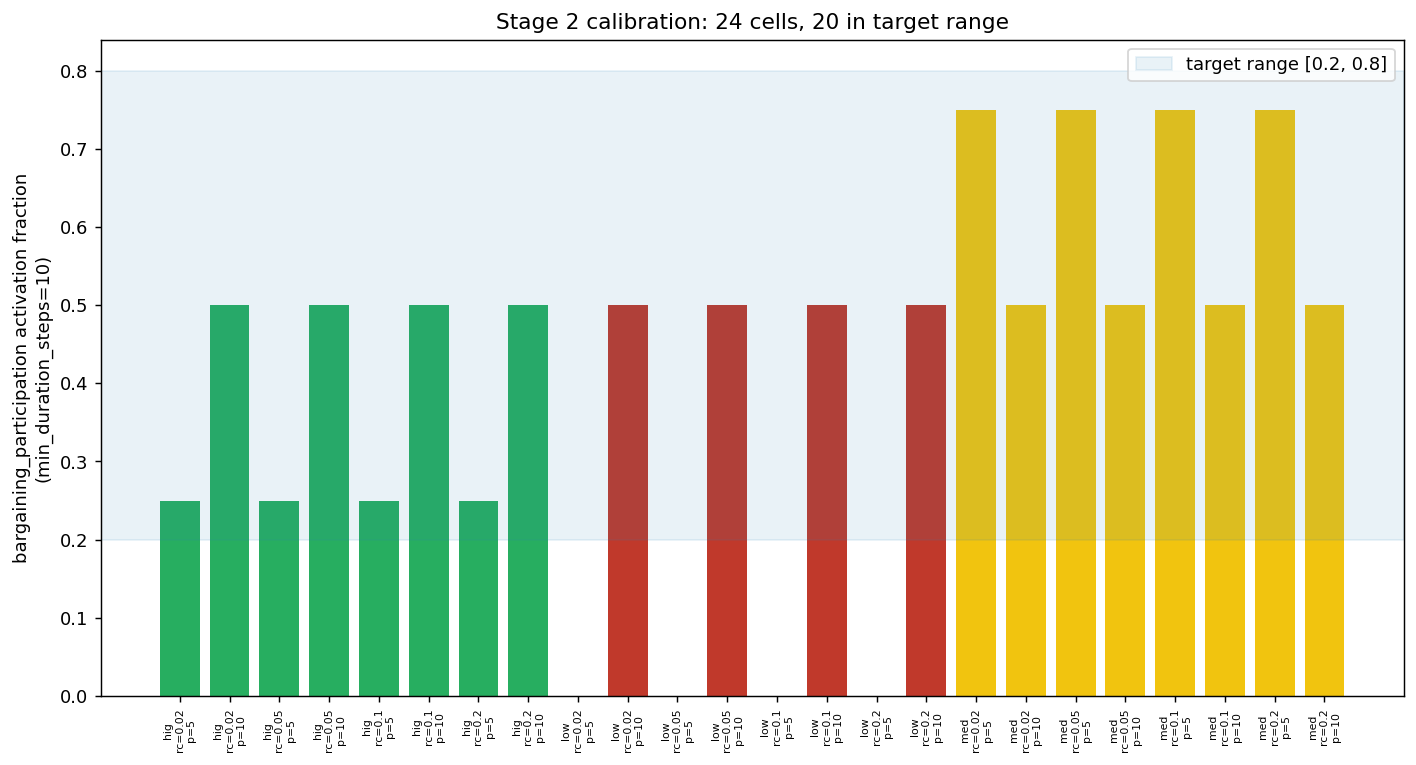
\includegraphics[width=0.75\textwidth]{figures/level13b/l13b_fig2_bargaining_activation.png}
\caption{Level 1.3b H1: bargaining-participation activation after the
Work Package B observer-construction fix. Stage 2 calibration (96 runs,
24 cells $\times$ 4 seeds): 20/24 cells land in the target $[0.2,0.8]$
activation range at unmodified Level 1.1/1.2b defaults.}
\label{fig:l13b-bargaining-activation}
\end{figure}

\begin{figure}[htbp]
\centering
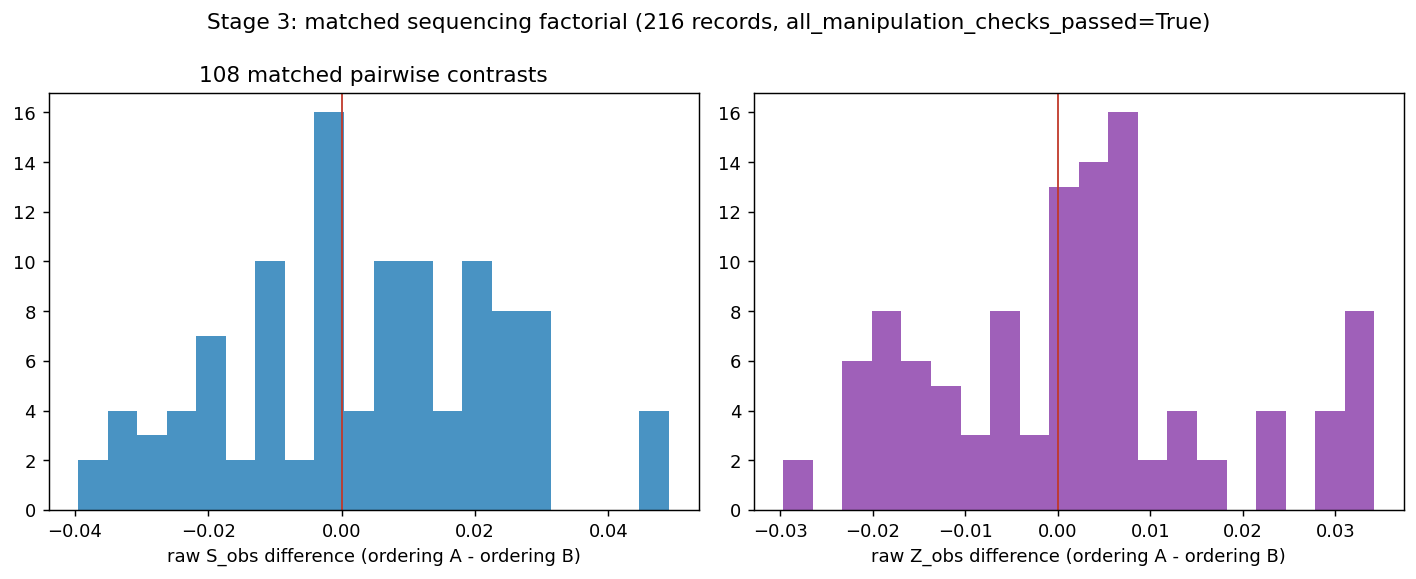
\includegraphics[width=0.85\textwidth]{figures/level13b/l13b_fig3_ordering_contrasts.png}
\caption{Level 1.3b H2: Stage 3 matched pairwise contrasts (216 runs, 108
matched pairwise comparisons per outcome variable), seed-clustered
bootstrap confidence intervals. 24.1\%/32.4\% of contrasts exclude zero on
$S_{\text{obs}}$/$Z_{\text{obs}}$; direction is not uniform across the
three ordering pairs.}
\label{fig:l13b-ordering}
\end{figure}

\begin{figure}[htbp]
\centering
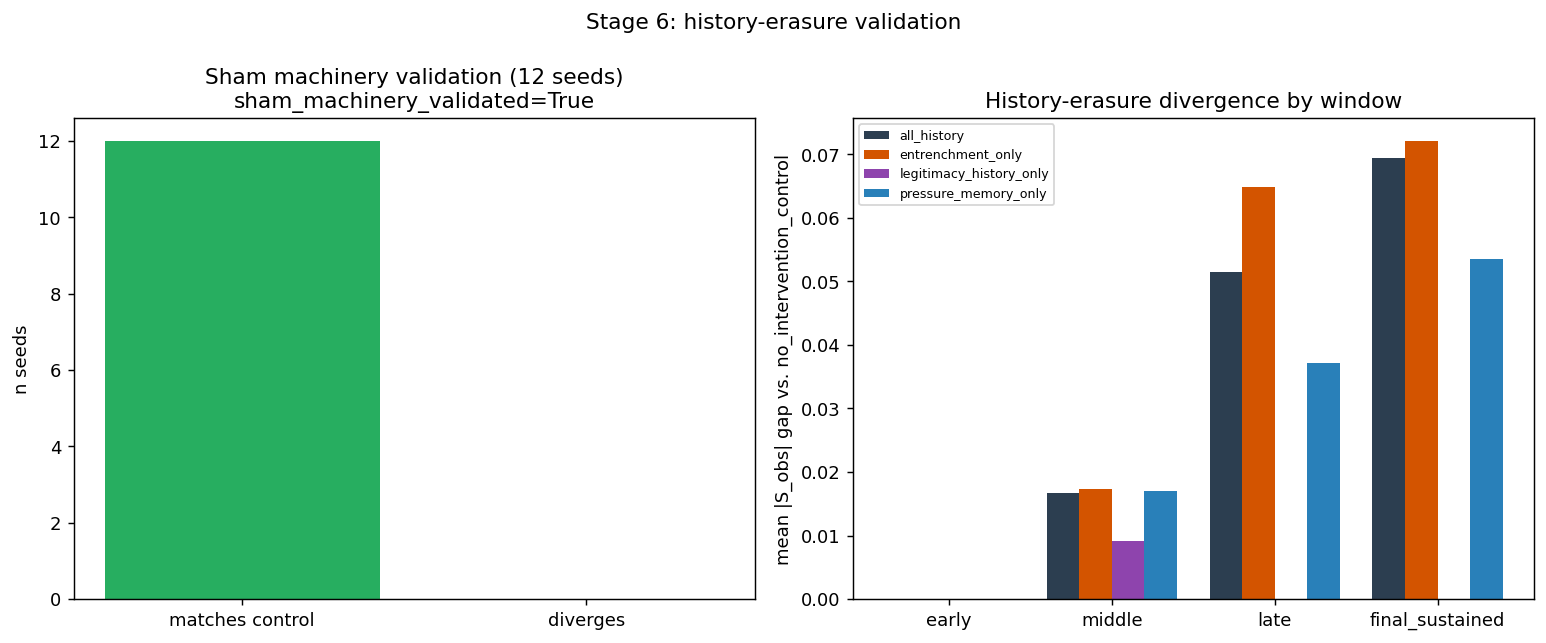
\includegraphics[width=0.9\textwidth]{figures/level13b/l13b_fig4_sham_and_divergence.png}
\caption{Level 1.3b H5: Stage 6 sham-machinery validation (left; 12/12
seeds byte-identical to control) and history-erasure divergence by window
(right; mean $|S_{\text{obs}}|$ gap versus control, four intervention arms
across early/middle/late/final-sustained windows). Every real intervention
except \texttt{legitimacy\_history\_only} shows a growing, non-decaying
gap. Causal evidence, sham-validated --- not a correlational sweep.}
\label{fig:l13b-sham}
\end{figure}

\begin{figure}[htbp]
\centering
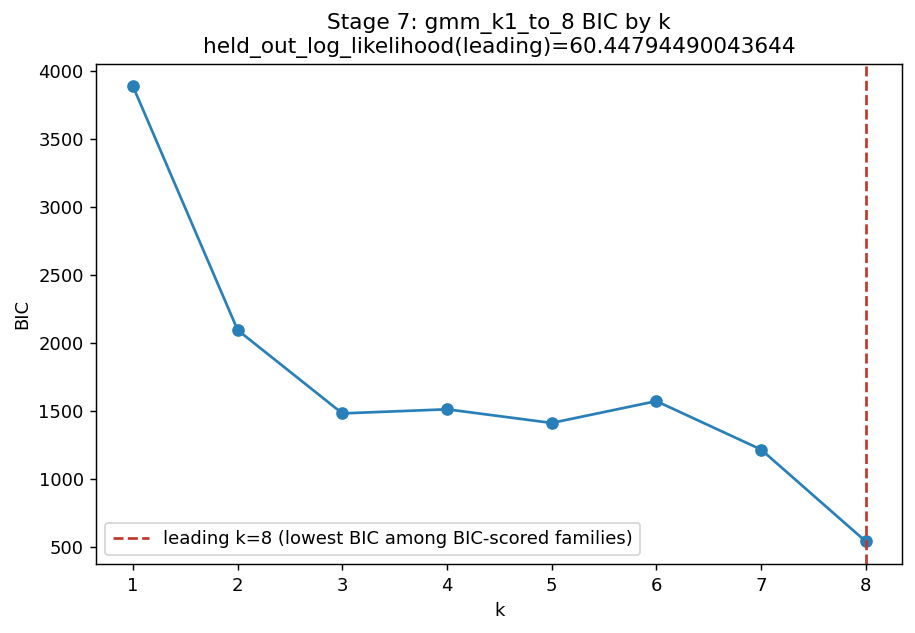
\includegraphics[width=0.75\textwidth]{figures/level13b/l13b_fig5a_bic_curve.png}
\caption{Level 1.3b Stage 7: Bayesian information criterion by $k$ for
\texttt{gmm\_k1\_to\_8} (240 pooled runs). Lowest (``leading'') BIC at
$k{=}8$, with a sharp, non-turning drop from $k{=}7$. \textbf{This BIC
curve alone does not establish eight institutional species}; read only
alongside \cref{fig:l13b-discreteness}'s weak cross-algorithm and
cross-stratum agreement and the silhouette values reported in
\cref{sec:level13b-h7h8}, which together indicate a still-improving
flexible density fit to a continuous, non-Gaussian distribution rather
than eight genuinely separated families.}
\label{fig:l13b-bic}
\end{figure}

\begin{figure}[htbp]
\centering
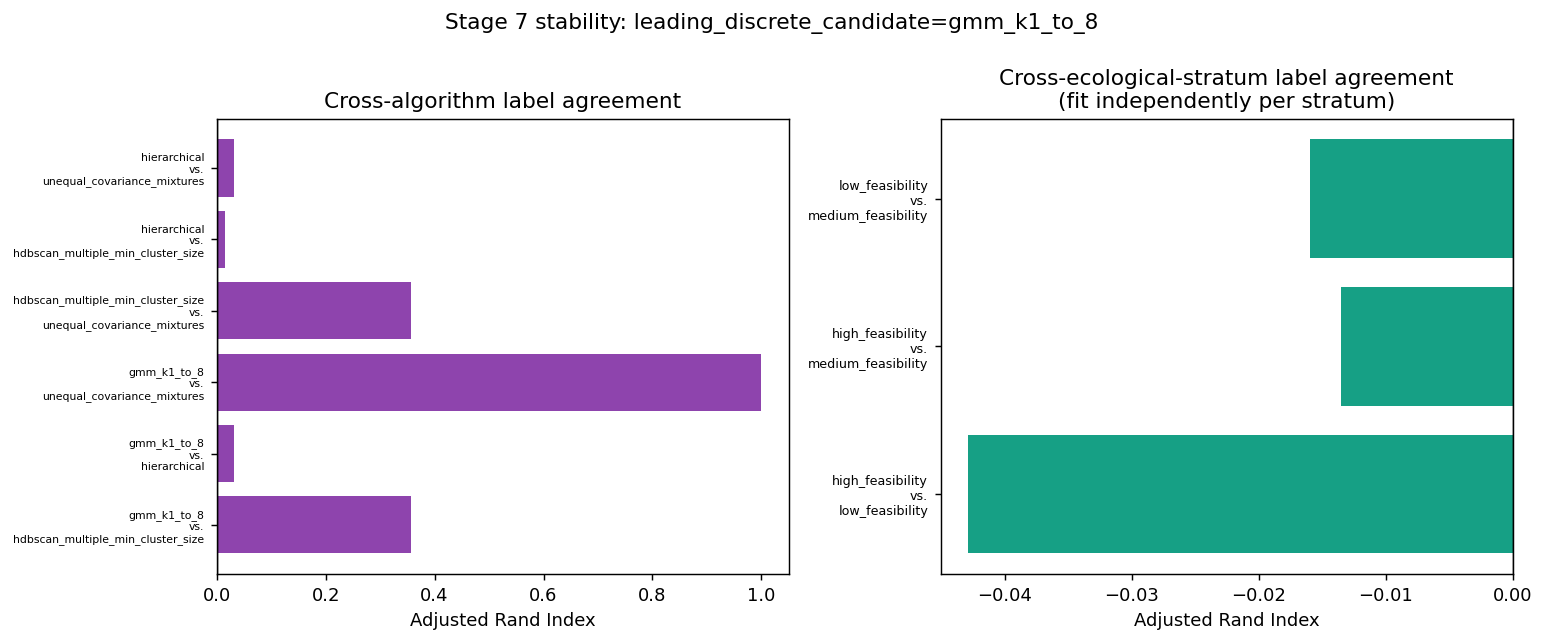
\includegraphics[width=0.95\textwidth]{figures/level13b/l13b_fig5b_discreteness_evidence.png}
\caption{Level 1.3b H8, evidence against discreteness at $k{=}8$: pairwise
cross-algorithm label agreement (left; weak, 0.016--0.357, once the
non-independent \texttt{gmm}/\texttt{unequal\_covariance\_mixtures} pair,
adjusted Rand index 1.0, is set aside) and cross-ecological-stratum label
agreement (right; near-zero to negative, $-0.043$ to $-0.014$, when the
leading method is refit independently within each stratum). Paired with
\cref{fig:l13b-bic} per this paper's own figure-pairing rule: mixture
components are not institutional species.}
\label{fig:l13b-discreteness}
\end{figure}

\begin{figure}[htbp]
\centering
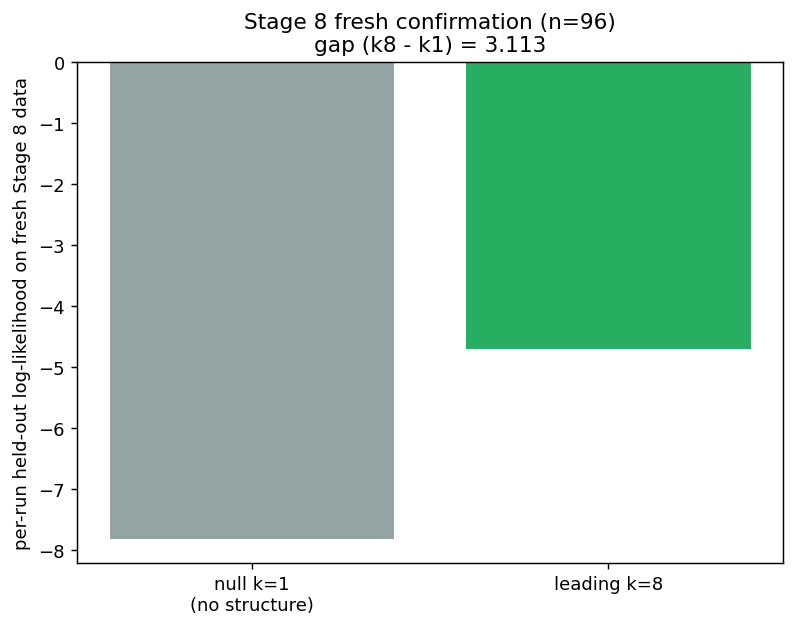
\includegraphics[width=0.6\textwidth]{figures/level13b/l13b_fig6_generalization_gap.png}
\caption{Level 1.3b H7: Stage 8 fresh-data generalization gap, leading
discrete candidate ($k{=}8$) per-run log-likelihood minus null ($k{=}1$)
per-run log-likelihood, 96-run disjoint fresh confirmation pool. Positive
($+3.11$), unlike Level 1.3's own sharply negative fresh-data collapse ---
but a weak discreteness signal alone, since the leading continuous
candidate also generalizes well (\cref{sec:level13b-h7h8}).}
\label{fig:l13b-generalization}
\end{figure}

\begin{figure}[htbp]
\centering
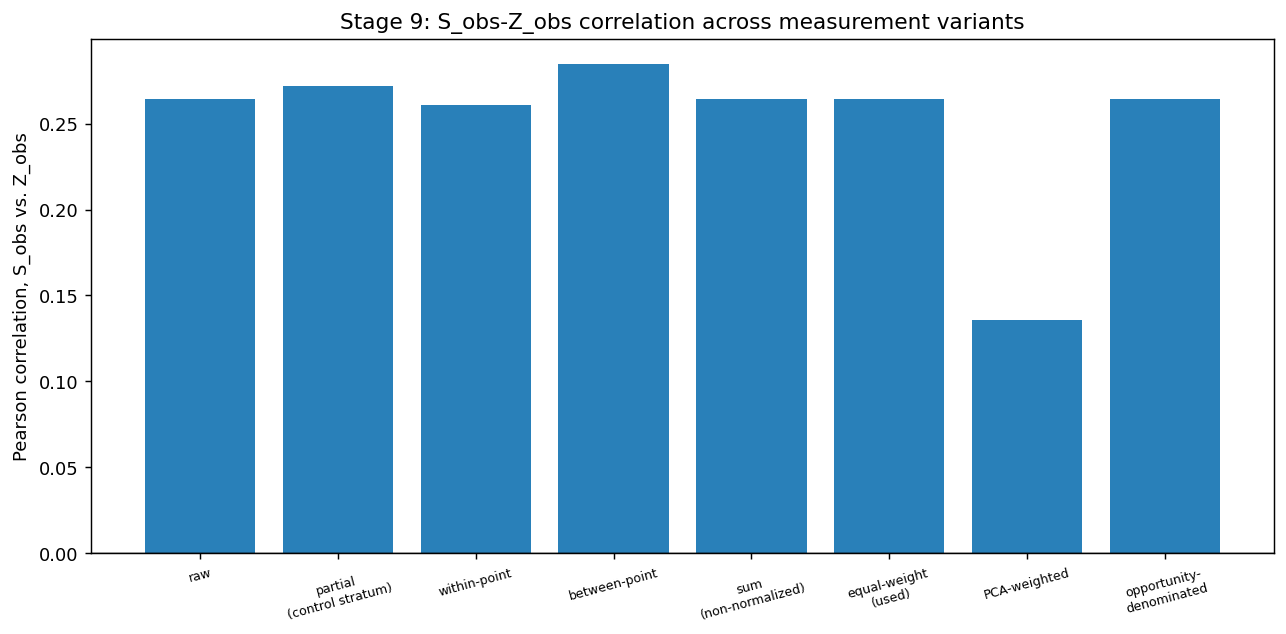
\includegraphics[width=0.85\textwidth]{figures/level13b/l13b_fig7_coupling_robustness.png}
\caption{Level 1.3b Stage 9: $S_{\text{obs}}$--$Z_{\text{obs}}$ correlation
across defensible measurement-weighting variants (equal-weight, partial
controlling ecological stratum, between-/within-point, leave-one-component-
out range, PCA-weighted). Equal-weight and related variants cluster near
$r\approx0.26$--$0.29$; the PCA-weighted alternative is a genuine outlier
at $r\approx0.14$, roughly half.}
\label{fig:l13b-coupling-robustness}
\end{figure}
